\documentclass{article}

%----------------------------------Packages------------------------------------%
\usepackage{graphicx, float}            % Graphics/Images.
\usepackage[dvipsnames]{xcolor}         % Color names.
\usepackage{mathtools, esint, mathrsfs} % amsmath and integrals.
\usepackage{amsthm, amsfonts, amssymb}  % Fonts and theorems.
\usepackage{pgfplots, tikz}             % Drawing/graphing tools.
\usepackage{graphicx, float}
\usetikzlibrary{arrows.meta, decorations.markings, positioning}

\newcommand{\interior}[2][\tau]{\mathrm{Int}_{#1}(#2)}
\DeclareMathSymbol{\minus}{\mathbin}{AMSa}{"39}

% \usetikzlibrary{
%     calc,                   % Calculating right angles and more.
%     angles,                 % Drawing angles within triangles.
%     arrows.meta,            % Latex and Stealth arrows.
%     quotes,                 % Adding labels to angles.
%     positioning,            % Relative positioning of nodes.
%     decorations.markings,   % Adding arrows in the middle of a line.
%     patterns,
%     arrows
% }
\pgfplotsset{compat=1.9}

\usepackage[pdftex,
            pdfauthor={Ryan Maguire},
            pdftitle={Tikz Gallery},
            pdfsubject={Mathematics, Physics, Science, Drawing, Figures},
            pdfkeywords={Mathematics, Physics, Tikz, Asymptote},
            pdfproducer={LaTeX},
            pdfcreator={pdflatex}]{hyperref}

% Colors for hyperref.
\hypersetup{colorlinks=true, linkcolor=blue}

\title{Tikz/Asymptote Gallery}
\author{Ryan Maguire}
\date{\today}
\begin{document}
    \maketitle
    \tableofcontents
    \listoffigures
    \newpage
    \section{Tikz}
        \begin{figure}[H]
            \centering
            \documentclass{standalone}
\usepackage{tikz}
\begin{document}
    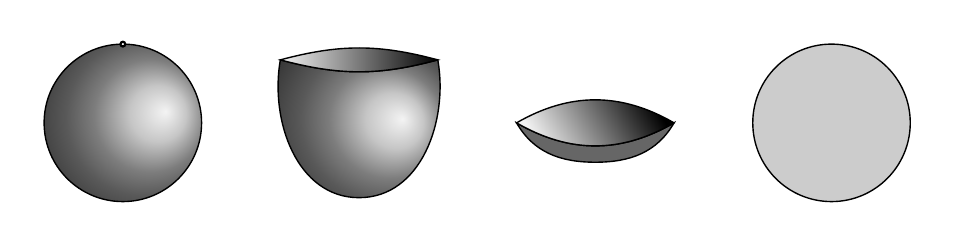
\begin{tikzpicture}[%
        scale=1,
        line width=0.5pt,
        sphereshade/.style={
            ball color=gray!60!white,
            draw=black,
            shading angle=240
        }
    ]
        % Some space to prevent clipping the image in the PDF.
        \draw[draw=white] (-5.2, -1.2) rectangle (6.2, 1.2);

        % Points for the Second Blob.
        \coordinate (a) at (-1.0, -0.95);
        \coordinate (b) at (-2.0,  0.80);
        \coordinate (c) at ( 0.0,  0.80);

        % Points for the Third Blob.
        \coordinate (d) at (2.0, -0.5);
        \coordinate (e) at (1.0,  0.0);
        \coordinate (f) at (3.0,  0.0);

        % First blob (Sphere).
        \filldraw[sphereshade] (-4,0) circle (1);

        % North pole of the sphere is missing.
        \filldraw[white, draw=black, thick] (-4,1) circle (0.3mm);

        % Draw the second blob
        \draw[sphereshade] (a) to [out=180,in=-100] (b)
                            to [out=-15,in=-165] (c)
                            to [out=-80,in=0] cycle;

        \draw[left color=white!90!gray,right color=black]
            (b) to [out=-15,in=-165] (c)
                to [out=165,in=15] cycle;

        % Draw the third blob
        \draw[fill=black!20!gray]
            (d) to [out=180,in=-60] (e) 
                to [out=-30,in=-150] (f)
                to [out=-120,in=0] cycle;
        \draw[left color=black, right color=white!90!gray,shading angle=300]
            (e) to [out=-30,in=-150] (f)
                to [out=150,in=30] cycle;

        % Draw the fourth blob (Circle)
        \filldraw[draw=black, fill=white!60!gray] (5,0) circle (1);
    \end{tikzpicture}
\end{document}
            \caption{\_\_Old\_Sphere\_to\_Disk\_Homeo.tex}
        \end{figure}
        \begin{figure}[H]
            \centering
            \documentclass[crop,class=article]{standalone}
%----------------------------Preamble-------------------------------%
%---------------------------Packages----------------------------%
\usepackage{geometry}
\geometry{b5paper, margin=1.0in}
\usepackage[T1]{fontenc}
\usepackage{graphicx, float}            % Graphics/Images.
\usepackage{natbib}                     % For bibliographies.
\bibliographystyle{agsm}                % Bibliography style.
\usepackage[french, english]{babel}     % Language typesetting.
\usepackage[dvipsnames]{xcolor}         % Color names.
\usepackage{listings}                   % Verbatim-Like Tools.
\usepackage{mathtools, esint, mathrsfs} % amsmath and integrals.
\usepackage{amsthm, amsfonts, amssymb}  % Fonts and theorems.
\usepackage{tcolorbox}                  % Frames around theorems.
\usepackage{upgreek}                    % Non-Italic Greek.
\usepackage{fmtcount, etoolbox}         % For the \book{} command.
\usepackage[newparttoc]{titlesec}       % Formatting chapter, etc.
\usepackage{titletoc}                   % Allows \book in toc.
\usepackage[nottoc]{tocbibind}          % Bibliography in toc.
\usepackage[titles]{tocloft}            % ToC formatting.
\usepackage{pgfplots, tikz}             % Drawing/graphing tools.
\usepackage{imakeidx}                   % Used for index.
\usetikzlibrary{
    calc,                   % Calculating right angles and more.
    angles,                 % Drawing angles within triangles.
    arrows.meta,            % Latex and Stealth arrows.
    quotes,                 % Adding labels to angles.
    positioning,            % Relative positioning of nodes.
    decorations.markings,   % Adding arrows in the middle of a line.
    patterns,
    arrows
}                                       % Libraries for tikz.
\pgfplotsset{compat=1.9}                % Version of pgfplots.
\usepackage[font=scriptsize,
            labelformat=simple,
            labelsep=colon]{subcaption} % Subfigure captions.
\usepackage[font={scriptsize},
            hypcap=true,
            labelsep=colon]{caption}    % Figure captions.
\usepackage[pdftex,
            pdfauthor={Ryan Maguire},
            pdftitle={Mathematics and Physics},
            pdfsubject={Mathematics, Physics, Science},
            pdfkeywords={Mathematics, Physics, Computer Science, Biology},
            pdfproducer={LaTeX},
            pdfcreator={pdflatex}]{hyperref}
\hypersetup{
    colorlinks=true,
    linkcolor=blue,
    filecolor=magenta,
    urlcolor=Cerulean,
    citecolor=SkyBlue
}                           % Colors for hyperref.
\usepackage[toc,acronym,nogroupskip,nopostdot]{glossaries}
\usepackage{glossary-mcols}
%------------------------Theorem Styles-------------------------%
\theoremstyle{plain}
\newtheorem{theorem}{Theorem}[section]

% Define theorem style for default spacing and normal font.
\newtheoremstyle{normal}
    {\topsep}               % Amount of space above the theorem.
    {\topsep}               % Amount of space below the theorem.
    {}                      % Font used for body of theorem.
    {}                      % Measure of space to indent.
    {\bfseries}             % Font of the header of the theorem.
    {}                      % Punctuation between head and body.
    {.5em}                  % Space after theorem head.
    {}

% Italic header environment.
\newtheoremstyle{thmit}{\topsep}{\topsep}{}{}{\itshape}{}{0.5em}{}

% Define environments with italic headers.
\theoremstyle{thmit}
\newtheorem*{solution}{Solution}

% Define default environments.
\theoremstyle{normal}
\newtheorem{example}{Example}[section]
\newtheorem{definition}{Definition}[section]
\newtheorem{problem}{Problem}[section]

% Define framed environment.
\tcbuselibrary{most}
\newtcbtheorem[use counter*=theorem]{ftheorem}{Theorem}{%
    before=\par\vspace{2ex},
    boxsep=0.5\topsep,
    after=\par\vspace{2ex},
    colback=green!5,
    colframe=green!35!black,
    fonttitle=\bfseries\upshape%
}{thm}

\newtcbtheorem[auto counter, number within=section]{faxiom}{Axiom}{%
    before=\par\vspace{2ex},
    boxsep=0.5\topsep,
    after=\par\vspace{2ex},
    colback=Apricot!5,
    colframe=Apricot!35!black,
    fonttitle=\bfseries\upshape%
}{ax}

\newtcbtheorem[use counter*=definition]{fdefinition}{Definition}{%
    before=\par\vspace{2ex},
    boxsep=0.5\topsep,
    after=\par\vspace{2ex},
    colback=blue!5!white,
    colframe=blue!75!black,
    fonttitle=\bfseries\upshape%
}{def}

\newtcbtheorem[use counter*=example]{fexample}{Example}{%
    before=\par\vspace{2ex},
    boxsep=0.5\topsep,
    after=\par\vspace{2ex},
    colback=red!5!white,
    colframe=red!75!black,
    fonttitle=\bfseries\upshape%
}{ex}

\newtcbtheorem[auto counter, number within=section]{fnotation}{Notation}{%
    before=\par\vspace{2ex},
    boxsep=0.5\topsep,
    after=\par\vspace{2ex},
    colback=SeaGreen!5!white,
    colframe=SeaGreen!75!black,
    fonttitle=\bfseries\upshape%
}{not}

\newtcbtheorem[use counter*=remark]{fremark}{Remark}{%
    fonttitle=\bfseries\upshape,
    colback=Goldenrod!5!white,
    colframe=Goldenrod!75!black}{ex}

\newenvironment{bproof}{\textit{Proof.}}{\hfill$\square$}
\tcolorboxenvironment{bproof}{%
    blanker,
    breakable,
    left=3mm,
    before skip=5pt,
    after skip=10pt,
    borderline west={0.6mm}{0pt}{green!80!black}
}

\AtEndEnvironment{lexample}{$\hfill\textcolor{red}{\blacksquare}$}
\newtcbtheorem[use counter*=example]{lexample}{Example}{%
    empty,
    title={Example~\theexample},
    boxed title style={%
        empty,
        size=minimal,
        toprule=2pt,
        top=0.5\topsep,
    },
    coltitle=red,
    fonttitle=\bfseries,
    parbox=false,
    boxsep=0pt,
    before=\par\vspace{2ex},
    left=0pt,
    right=0pt,
    top=3ex,
    bottom=1ex,
    before=\par\vspace{2ex},
    after=\par\vspace{2ex},
    breakable,
    pad at break*=0mm,
    vfill before first,
    overlay unbroken={%
        \draw[red, line width=2pt]
            ([yshift=-1.2ex]title.south-|frame.west) to
            ([yshift=-1.2ex]title.south-|frame.east);
        },
    overlay first={%
        \draw[red, line width=2pt]
            ([yshift=-1.2ex]title.south-|frame.west) to
            ([yshift=-1.2ex]title.south-|frame.east);
    },
}{ex}

\AtEndEnvironment{ldefinition}{$\hfill\textcolor{Blue}{\blacksquare}$}
\newtcbtheorem[use counter*=definition]{ldefinition}{Definition}{%
    empty,
    title={Definition~\thedefinition:~{#1}},
    boxed title style={%
        empty,
        size=minimal,
        toprule=2pt,
        top=0.5\topsep,
    },
    coltitle=Blue,
    fonttitle=\bfseries,
    parbox=false,
    boxsep=0pt,
    before=\par\vspace{2ex},
    left=0pt,
    right=0pt,
    top=3ex,
    bottom=0pt,
    before=\par\vspace{2ex},
    after=\par\vspace{1ex},
    breakable,
    pad at break*=0mm,
    vfill before first,
    overlay unbroken={%
        \draw[Blue, line width=2pt]
            ([yshift=-1.2ex]title.south-|frame.west) to
            ([yshift=-1.2ex]title.south-|frame.east);
        },
    overlay first={%
        \draw[Blue, line width=2pt]
            ([yshift=-1.2ex]title.south-|frame.west) to
            ([yshift=-1.2ex]title.south-|frame.east);
    },
}{def}

\AtEndEnvironment{ltheorem}{$\hfill\textcolor{Green}{\blacksquare}$}
\newtcbtheorem[use counter*=theorem]{ltheorem}{Theorem}{%
    empty,
    title={Theorem~\thetheorem:~{#1}},
    boxed title style={%
        empty,
        size=minimal,
        toprule=2pt,
        top=0.5\topsep,
    },
    coltitle=Green,
    fonttitle=\bfseries,
    parbox=false,
    boxsep=0pt,
    before=\par\vspace{2ex},
    left=0pt,
    right=0pt,
    top=3ex,
    bottom=-1.5ex,
    breakable,
    pad at break*=0mm,
    vfill before first,
    overlay unbroken={%
        \draw[Green, line width=2pt]
            ([yshift=-1.2ex]title.south-|frame.west) to
            ([yshift=-1.2ex]title.south-|frame.east);},
    overlay first={%
        \draw[Green, line width=2pt]
            ([yshift=-1.2ex]title.south-|frame.west) to
            ([yshift=-1.2ex]title.south-|frame.east);
    }
}{thm}

%--------------------Declared Math Operators--------------------%
\DeclareMathOperator{\adjoint}{adj}         % Adjoint.
\DeclareMathOperator{\Card}{Card}           % Cardinality.
\DeclareMathOperator{\curl}{curl}           % Curl.
\DeclareMathOperator{\diam}{diam}           % Diameter.
\DeclareMathOperator{\dist}{dist}           % Distance.
\DeclareMathOperator{\Div}{div}             % Divergence.
\DeclareMathOperator{\Erf}{Erf}             % Error Function.
\DeclareMathOperator{\Erfc}{Erfc}           % Complementary Error Function.
\DeclareMathOperator{\Ext}{Ext}             % Exterior.
\DeclareMathOperator{\GCD}{GCD}             % Greatest common denominator.
\DeclareMathOperator{\grad}{grad}           % Gradient
\DeclareMathOperator{\Ima}{Im}              % Image.
\DeclareMathOperator{\Int}{Int}             % Interior.
\DeclareMathOperator{\LC}{LC}               % Leading coefficient.
\DeclareMathOperator{\LCM}{LCM}             % Least common multiple.
\DeclareMathOperator{\LM}{LM}               % Leading monomial.
\DeclareMathOperator{\LT}{LT}               % Leading term.
\DeclareMathOperator{\Mod}{mod}             % Modulus.
\DeclareMathOperator{\Mon}{Mon}             % Monomial.
\DeclareMathOperator{\multideg}{mutlideg}   % Multi-Degree (Graphs).
\DeclareMathOperator{\nul}{nul}             % Null space of operator.
\DeclareMathOperator{\Ord}{Ord}             % Ordinal of ordered set.
\DeclareMathOperator{\Prin}{Prin}           % Principal value.
\DeclareMathOperator{\proj}{proj}           % Projection.
\DeclareMathOperator{\Refl}{Refl}           % Reflection operator.
\DeclareMathOperator{\rk}{rk}               % Rank of operator.
\DeclareMathOperator{\sgn}{sgn}             % Sign of a number.
\DeclareMathOperator{\sinc}{sinc}           % Sinc function.
\DeclareMathOperator{\Span}{Span}           % Span of a set.
\DeclareMathOperator{\Spec}{Spec}           % Spectrum.
\DeclareMathOperator{\supp}{supp}           % Support
\DeclareMathOperator{\Tr}{Tr}               % Trace of matrix.
%--------------------Declared Math Symbols--------------------%
\DeclareMathSymbol{\minus}{\mathbin}{AMSa}{"39} % Unary minus sign.
%------------------------New Commands---------------------------%
\DeclarePairedDelimiter\norm{\lVert}{\rVert}
\DeclarePairedDelimiter\ceil{\lceil}{\rceil}
\DeclarePairedDelimiter\floor{\lfloor}{\rfloor}
\newcommand*\diff{\mathop{}\!\mathrm{d}}
\newcommand*\Diff[1]{\mathop{}\!\mathrm{d^#1}}
\renewcommand*{\glstextformat}[1]{\textcolor{RoyalBlue}{#1}}
\renewcommand{\glsnamefont}[1]{\textbf{#1}}
\renewcommand\labelitemii{$\circ$}
\renewcommand\thesubfigure{%
    \arabic{chapter}.\arabic{figure}.\arabic{subfigure}}
\addto\captionsenglish{\renewcommand{\figurename}{Fig.}}
\numberwithin{equation}{section}

\renewcommand{\vector}[1]{\boldsymbol{\mathrm{#1}}}

\newcommand{\uvector}[1]{\boldsymbol{\hat{\mathrm{#1}}}}
\newcommand{\topspace}[2][]{(#2,\tau_{#1})}
\newcommand{\measurespace}[2][]{(#2,\varSigma_{#1},\mu_{#1})}
\newcommand{\measurablespace}[2][]{(#2,\varSigma_{#1})}
\newcommand{\manifold}[2][]{(#2,\tau_{#1},\mathcal{A}_{#1})}
\newcommand{\tanspace}[2]{T_{#1}{#2}}
\newcommand{\cotanspace}[2]{T_{#1}^{*}{#2}}
\newcommand{\Ckspace}[3][\mathbb{R}]{C^{#2}(#3,#1)}
\newcommand{\funcspace}[2][\mathbb{R}]{\mathcal{F}(#2,#1)}
\newcommand{\smoothvecf}[1]{\mathfrak{X}(#1)}
\newcommand{\smoothonef}[1]{\mathfrak{X}^{*}(#1)}
\newcommand{\bracket}[2]{[#1,#2]}

%------------------------Book Command---------------------------%
\makeatletter
\renewcommand\@pnumwidth{1cm}
\newcounter{book}
\renewcommand\thebook{\@Roman\c@book}
\newcommand\book{%
    \if@openright
        \cleardoublepage
    \else
        \clearpage
    \fi
    \thispagestyle{plain}%
    \if@twocolumn
        \onecolumn
        \@tempswatrue
    \else
        \@tempswafalse
    \fi
    \null\vfil
    \secdef\@book\@sbook
}
\def\@book[#1]#2{%
    \refstepcounter{book}
    \addcontentsline{toc}{book}{\bookname\ \thebook:\hspace{1em}#1}
    \markboth{}{}
    {\centering
     \interlinepenalty\@M
     \normalfont
     \huge\bfseries\bookname\nobreakspace\thebook
     \par
     \vskip 20\p@
     \Huge\bfseries#2\par}%
    \@endbook}
\def\@sbook#1{%
    {\centering
     \interlinepenalty \@M
     \normalfont
     \Huge\bfseries#1\par}%
    \@endbook}
\def\@endbook{
    \vfil\newpage
        \if@twoside
            \if@openright
                \null
                \thispagestyle{empty}%
                \newpage
            \fi
        \fi
        \if@tempswa
            \twocolumn
        \fi
}
\newcommand*\l@book[2]{%
    \ifnum\c@tocdepth >-3\relax
        \addpenalty{-\@highpenalty}%
        \addvspace{2.25em\@plus\p@}%
        \setlength\@tempdima{3em}%
        \begingroup
            \parindent\z@\rightskip\@pnumwidth
            \parfillskip -\@pnumwidth
            {
                \leavevmode
                \Large\bfseries#1\hfill\hb@xt@\@pnumwidth{\hss#2}
            }
            \par
            \nobreak
            \global\@nobreaktrue
            \everypar{\global\@nobreakfalse\everypar{}}%
        \endgroup
    \fi}
\newcommand\bookname{Book}
\renewcommand{\thebook}{\texorpdfstring{\Numberstring{book}}{book}}
\providecommand*{\toclevel@book}{-2}
\makeatother
\titleformat{\part}[display]
    {\Large\bfseries}
    {\partname\nobreakspace\thepart}
    {0mm}
    {\Huge\bfseries}
\titlecontents{part}[0pt]
    {\large\bfseries}
    {\partname\ \thecontentslabel: \quad}
    {}
    {\hfill\contentspage}
\titlecontents{chapter}[0pt]
    {\bfseries}
    {\chaptername\ \thecontentslabel:\quad}
    {}
    {\hfill\contentspage}
\newglossarystyle{longpara}{%
    \setglossarystyle{long}%
    \renewenvironment{theglossary}{%
        \begin{longtable}[l]{{p{0.25\hsize}p{0.65\hsize}}}
    }{\end{longtable}}%
    \renewcommand{\glossentry}[2]{%
        \glstarget{##1}{\glossentryname{##1}}%
        &\glossentrydesc{##1}{~##2.}
        \tabularnewline%
        \tabularnewline
    }%
}
\newglossary[not-glg]{notation}{not-gls}{not-glo}{Notation}
\newcommand*{\newnotation}[4][]{%
    \newglossaryentry{#2}{type=notation, name={\textbf{#3}, },
                          text={#4}, description={#4},#1}%
}
%--------------------------LENGTHS------------------------------%
% Spacings for the Table of Contents.
\addtolength{\cftsecnumwidth}{1ex}
\addtolength{\cftsubsecindent}{1ex}
\addtolength{\cftsubsecnumwidth}{1ex}
\addtolength{\cftfignumwidth}{1ex}
\addtolength{\cfttabnumwidth}{1ex}

% Indent and paragraph spacing.
\setlength{\parindent}{0em}
\setlength{\parskip}{0em}
%--------------------------Main Document----------------------------%
\begin{document}
    \begin{tikzpicture}[line cap=round,>={Stealth[black]}]
        \begin{scope}[
            every node/.style={
                circle,
                fill=black,
                draw=black,
                inner sep=0pt,
                minimum size=3pt
            }
        ]
            \node (A) at (3.5,0) {};
            \node (B) at (-3,1.5) {};
        \end{scope}
        \path[very thick,->,draw=red] (A) edge[bend right=15] (B);
        \draw[fill=blue,path fading=ringo,]
            (0,0) circle (15mm) (0,0) circle (1.2cm);
        \draw[inner color=white,outer color=black!100!gray]
            (0, 0) circle (1.2cm);
    \end{tikzpicture}
\end{document}
            \caption{Atmospheric\_Occultation.tex}
        \end{figure}
        \begin{figure}[H]
            \centering
            %--------------------------------Dependencies----------------------------------%
%   tikz                                                                       %
%       arrows.meta                                                            %
%-------------------------------Main Document----------------------------------%
\begin{tikzpicture}[%
    >=Latex,
    line width=0.2mm,
    line cap=round,
    scale=1.7
]

    % Coordinates for the various points.
    \coordinate (O)   at (0.0, 0.0);
    \coordinate (P)   at (4.0, 4.0);

    % Axes:
    \begin{scope}[thick, ->]
        \draw (-0.5,  0.0) to (4.4, 0.0) node [above] {$x$};
        \draw ( 0.0, -0.5) to (0.0, 4.4) node [right] {$y$};
    \end{scope}

    % Draw the main part of the function.
    \draw (O) to (P);

    % Draw a dot marking f(0).
    \draw[fill=black, draw=black] (0, 0.5in) circle (0.3mm);

    % Draw the rest of the function.
    \foreach\x in{4, 2, 1, 0.5, 0.25, 0.125}{
        \draw[fill=white, draw=black] (\x, \x) circle (0.3mm);
        \draw[fill=black, draw=black] (\x, 0.25*\x) circle (0.3mm);
    }
\end{tikzpicture}
            \caption{Bijection\_Closed\_to\_Open\_Interval.tex}
        \end{figure}
        \begin{figure}[H]
            \centering
            %--------------------------------Dependencies----------------------------------%
%   tikz                                                                       %
%-------------------------------Main Document----------------------------------%
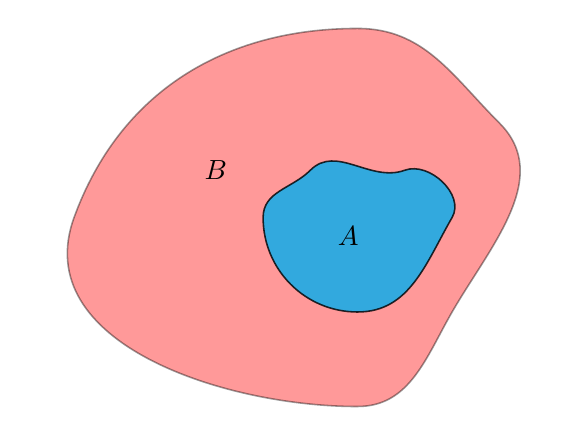
\begin{tikzpicture}[line width=0.2mm, scale=1.2]

    % Coordinates for the bigger blob.
    \coordinate (P1) at ( 0.0, -2.0);
    \coordinate (P2) at ( 1.0, -1.0);
    \coordinate (P3) at ( 1.5,  1.0);
    \coordinate (P4) at ( 0.0,  2.0);
    \coordinate (P5) at (-3.0,  0.0);

    % Coordinates for the inner blob.
    \coordinate (Q1) at ( 0.0, -1.0);
    \coordinate (Q2) at ( 1.0,  0.0);
    \coordinate (Q3) at ( 0.5,  0.5);
    \coordinate (Q4) at (-0.5,  0.5);
    \coordinate (Q5) at (-1.0,  0.0);

    % Coordindates to label things.
    \coordinate (A) at (-0.1, -0.2);
    \coordinate (B) at (-1.5,  0.5);

    % Draw the bigger blob.
    \draw[fill=red, opacity=0.4] (P1) to [out=0,    in=-120] (P2)
                                      to [out=60,   in=-45]  (P3)
                                      to [out=135,  in=0]    (P4)
                                      to [out=-180, in=70]   (P5)
                                      to [out=-110, in=-180] cycle;

    % Draw the inner blob.
    \draw[fill=cyan, opacity=0.8] (Q1) to [out=0,    in=-120]  (Q2)
                                       to [out=60,   in=20]    (Q3)
                                       to [out=-160, in=45]    (Q4)
                                       to [out=-135, in=90]    (Q5)
                                       to [out=-90,  in=180]   cycle;

    % Labels for the two blobs.
    \node at (A) {$A$};
    \node at (B) {$B$};
\end{tikzpicture}

            \caption{Blobs\_Subset\_Example\_001.tex}
        \end{figure}
        \begin{figure}[H]
            \centering
            %--------------------------------Dependencies----------------------------------%
%   tikz                                                                       %
%       arrows.meta                                                            %
%-------------------------------Main Document----------------------------------%
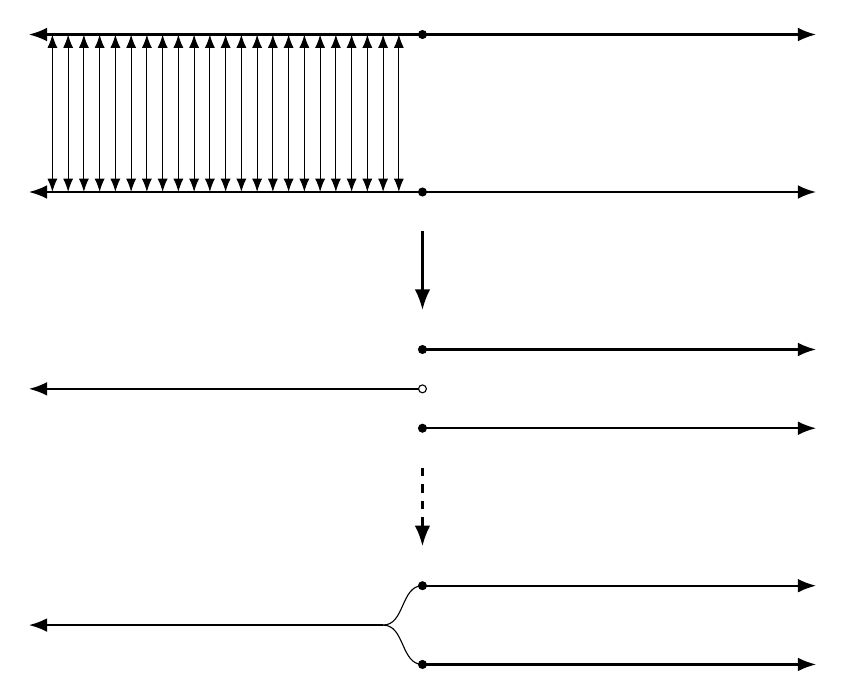
\begin{tikzpicture}[>=Latex]
    % Draw axes for the upper and lower lines. (First figure).
    \draw[<->, thick] (-5, 0) to (5, 0);
    \draw[<->, thick] (-5, 2) to (5, 2);

    % Connect the dots for all points to the left of the two origins.
    \foreach\x in {-4.7, -4.5, ..., -0.3}{
        \draw[<->] (\x, 2) to (\x, 0);
    }

    % Fill in circles for the two origins.
    \draw[fill=black] (0, 0) circle (0.5mm);
    \draw[fill=black] (0, 2) circle (0.5mm);

    % Draw a solid arrow to the next graphic.
    \draw [->, line width=1pt] (0, -0.5) to (0, -1.5);

    % Draw the second figure, shifted 2.5cm downwards.
    \begin{scope}[yshift=-2.5cm]

        % Draw the x-axis in the quotient space.
        \draw[<-, thick] (-5.0,  0.0) to (0.0,  0.0);
        \draw[->, thick] ( 0.0,  0.5) to (5.0,  0.5);
        \draw[->, thick] ( 0.0, -0.5) to (5.0, -0.5);

        % Remove the origin.
        \draw[fill=white, draw=black] (0, 0) circle (0.5mm);

        % Draw circles symbolizing the two origins.
        \draw[fill=black] (0.0,  0.5) circle (0.5mm);
        \draw[fill=black] (0.0, -0.5) circle (0.5mm);

        % Dashed arrow to the next graphic.
        \draw [->, line width=1pt, dashed] (0.0, -1.0) to (0.0, -2.0);
    \end{scope}

    % Draw the third figure (shift 5.5cm downwards).
    \begin{scope}[yshift=-5.5cm]

        % Draw the x-axis.
        \draw[<-, thick] (-5.0,  0.0) to (-0.5,  0.0);
        \draw[->, thick] ( 0.0,  0.5) to ( 5.0,  0.5);
        \draw[->, thick] ( 0.0, -0.5) to ( 5.0, -0.5);

        % Draw a curved line connecting the x-axis to the upper origin.
        \draw (-0.5, 0.0) to[out=0,in=180] (0.0, -0.5);

        % Draw a curved line connecting the x-axis to the lower origin.
        \draw (-0.5, 0.0) to[out=0,in=180] (0.0, 0.5);

        % Fill in the two origins.
        \draw[fill=black] (0.0,  0.5) circle (0.5mm);
        \draw[fill=black] (0.0, -0.5) circle (0.5mm);
    \end{scope}
\end{tikzpicture}
            \caption{Branching\_Line\_Construction.tex}
        \end{figure}
        \begin{figure}[H]
            \centering
            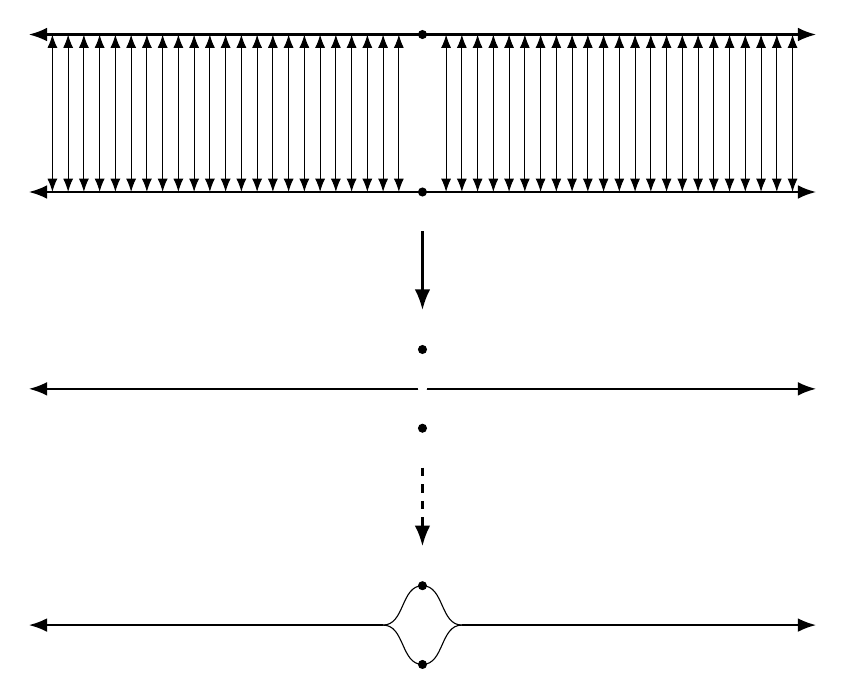
\begin{tikzpicture}[>=Latex]
    % Draw axes for the upper and lower lines (First figure).
    \draw[<->, thick] (-5, 0) to (5, 0);
    \draw[<->, thick] (-5, 2) to (5, 2);

    % Connect the dots for all points except for the two origins.
    \foreach\x in {-4.7, -4.5, ..., -0.3, 0.3, 0.5, ..., 4.7}{
        \draw[<->] (\x, 2) to (\x, 0);
    }

    % Fill in circles for the two origins.
    \draw[fill=black] (0, 0) circle (0.5mm);
    \draw[fill=black] (0, 2) circle (0.5mm);

    % Draw a solid arrow to the next graphic.
    \draw [->, line width=1pt] (0, -0.5) to (0, -1.5);

    % Draw the second figure shifted 2.5cm downwards.
    \begin{scope}[yshift=-2.5cm]
        % Draw the x-axis in the quotient space.
        \draw[<->, thick] (-5.0, 0.0) to (5.0, 0.0);

        % Remove the origin.
        \draw[fill=white, draw=white] (0, 0) circle (0.5mm);

        % Draw circles symbolizing the two origins.
        \draw[fill=black] (0.0,  0.5) circle (0.5mm);
        \draw[fill=black] (0.0, -0.5) circle (0.5mm);

        % Dashed arrow to the next graphic.
        \draw [->, line width=1pt, dashed] (0.0, -1.0) to (0.0, -2.0);
    \end{scope}

    % Draw the third figure shifted 5.5cm downwards.
    \begin{scope}[yshift=-5.5cm]
        % Draw the x-axis.
        \draw[<-, thick] (-5.0, 0.0) to (-0.5, 0);
        \draw[->, thick] ( 0.5, 0.0) to ( 5.0, 0);

        % Draw a curved line connecting the x-axis to the upper origin.
        \draw (-0.5, 0.0) to[out=0,in=180] (0.0, -0.5)
                          to[out=0,in=180] (0.5,  0.0);

        % Draw a curved line connecting the x-axis to the lower origin.
        \draw (-0.5, 0.0) to[out=0,in=180] (0.0, 0.5)
                          to[out=0,in=180] (0.5, 0.0);

        % Fill in the two origins.
        \draw[fill=black] (0.0,  0.5) circle (0.5mm);
        \draw[fill=black] (0.0, -0.5) circle (0.5mm);
    \end{scope}
\end{tikzpicture}
            \caption{Bug\_Eyed\_Line\_Construction.tex}
        \end{figure}
        \begin{figure}[H]
            \centering
            \begin{tikzpicture}[>=Latex]
    % Draw the x-axis.
    \draw[<-] (-5.0, 0.0) to (-0.5, 0.0);
    \draw[->] ( 0.5, 0.0) to ( 5.0, 0.0);

    % Shade an interval around the bottom origin.
    \draw[blue] (-0.5, 0.0) to[out=0,in=180] (0.0, -0.5)
                            to[out=0,in=180] (0.5,  0.0);

    % Connect the x-axis to the top origin.
    \draw (-0.5, 0.0) to[out=0,in=180] (0.0, 0.5)
                      to[out=0,in=180] (0.5, 0.0);

    % Shade the lower origin black, indicating it is not in the set.
    \draw[fill=black] (0.0,  0.5) circle (0.5mm);

    % Shade the upper origin blue, indicating is belongs to the set.
    \draw[fill=blue]  (0.0, -0.5) circle (0.5mm);

    % Label for the set U_0.
    \node at (2, 0.5) {$\mathcal{U}_{0}$};

    \begin{scope}[yshift=-2cm]
        % Draw the x-axis.
        \draw[<-] (-5.0, 0) to (-0.5, 0);
        \draw[->] ( 0.5, 0) to ( 5.0, 0);

        % Connect the lower origin to the x-axis.
        \draw (-0.5, 0.0) to[out=0,in=180] (0.0, -0.5)
                          to[out=0,in=180] (0.5,  0.0);

        % Shade an interval around the upper origin.
        \draw[blue] (-0.5, 0.0) to[out=0,in=180] (0.0, 0.5)
                                to[out=0,in=180] (0.5, 0.0);

        % Color the two origins accordingly.
        \draw[fill=blue]  (0.0,  0.5) circle (0.5mm);
        \draw[fill=black] (0.0, -0.5) circle (0.5mm);

        % Label for the set U_1.
        \node at (2, 0.5) {$\mathcal{U}_{1}$};
    \end{scope}

    \begin{scope}[yshift=-4cm]
        % Draw the x-axis.
        \draw[<-] (-5.0, 0) to (-0.5, 0);
        \draw[->] ( 0.5, 0) to ( 5.0, 0);

        % Blue coloring for the intersection of U_0 and U_1.
        \draw[blue, thick] (-0.5, 0) to (0.5, 0);

        % Delete the origin from this line.
        \draw[fill=white, draw=white] (0, 0) circle (0.5mm);

        % Color the two origins black.
        \draw[fill=black] (0,  0.5) circle (0.5mm);
        \draw[fill=black] (0, -0.5) circle (0.5mm);

        % Label for the intersection of U_0 and U_1.
        \node at (2, 0.5) {$\mathcal{U}_{0}\cap\mathcal{U}_{1}$};
    \end{scope}
\end{tikzpicture}
            \caption{Bug\_Eyed\_Line\_Open\_Sets.tex}
        \end{figure}
        \begin{figure}[H]
            \centering
            %--------------------------------Dependencies----------------------------------%
%   amssymb                                                                    %
%   tikz                                                                       %
%       arrows.meta                                                            %
%-------------------------------Main Document----------------------------------%
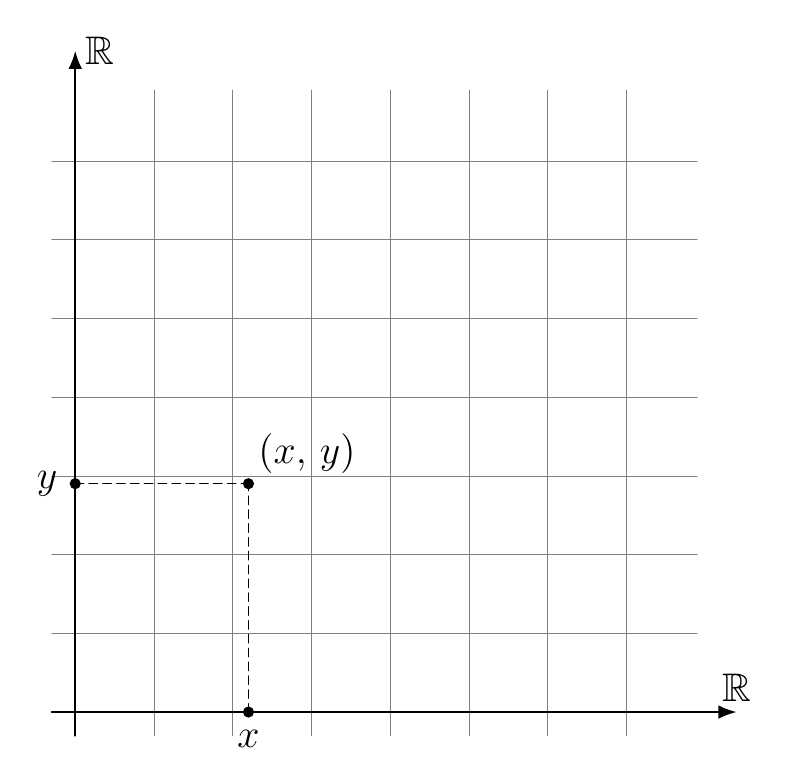
\begin{tikzpicture}[%
    >=Latex,
    line width=0.2mm,
    line cap=round,
    font=\Large
]
    % Coordinates for the points.
    \coordinate (x) at (2.2, 0.0);
    \coordinate (y) at (0.0, 2.9);
    \coordinate (z) at (2.2, 2.9);

    % Draw a grid.
    \draw[style=help lines] (-0.3, -0.3) grid (7.9, 7.9);

    % Axes.
    \begin{scope}[thick]
        \draw[->] (-0.3, 0) to (8.4, 0) node [above] {$\mathbb{R}$};
        \draw[->] (0, -0.3) to (0, 8.4) node [right] {$\mathbb{R}$};
    \end{scope}

    % Draw dashed lines to the point.
    \begin{scope}[densely dashed]
        \draw (x) to (z);
        \draw (y) to (z);
    \end{scope}

    % Draw dots marking the various points.
    \draw[fill=black] (x) circle (0.6mm);
    \draw[fill=black] (y) circle (0.6mm);
    \draw[fill=black] (z) circle (0.6mm);

    \node at (x) [below=0.1]     {$x$};
    \node at (y) [left=0.1]      {$y$};
    \node at (z) [above right]   {$(x,\,y)$};
\end{tikzpicture}
            \caption{Cartesian\_Product\_001.tex}
        \end{figure}
        \begin{figure}[H]
            \centering
            %--------------------------------Dependencies----------------------------------%
%   amssymb                                                                    %
%   tikz                                                                       %
%       arrows.meta                                                            %
%-------------------------------Main Document----------------------------------%
\begin{tikzpicture}[%
    >=Latex,
    line width=0.2mm,
    line cap=round
]

    % Axes.
    \begin{scope}[thick, font=\Large]
        \draw[->] (0, 0) to (8.4, 0) node [above] {$\mathbb{N}$};
        \draw[->] (0, 0) to (0, 8.4) node [right] {$\mathbb{N}$};
    \end{scope}

    \foreach\x in{1, 2, 3, 4, 5, 6, 7, 8}{
        \foreach\y in{1, 2, 3, 4, 5, 6, 7, 8}{
            \draw[fill=black] (\x, \y) circle (0.2mm);
        }
        \draw (\x, -0.1) to (\x, 0.1) node [below=1ex] {$\x$};
        \draw (-0.1, \x) to (0.1, \x) node [left=1ex]  {$\x$};
    }
\end{tikzpicture}
            \caption{Cartesian\_Product\_002.tex}
        \end{figure}
        \begin{figure}[H]
            \centering
            %--------------------------------Dependencies----------------------------------%
%   tikz                                                                       %
%       arrows.meta                                                            %
%-------------------------------Main Document----------------------------------%
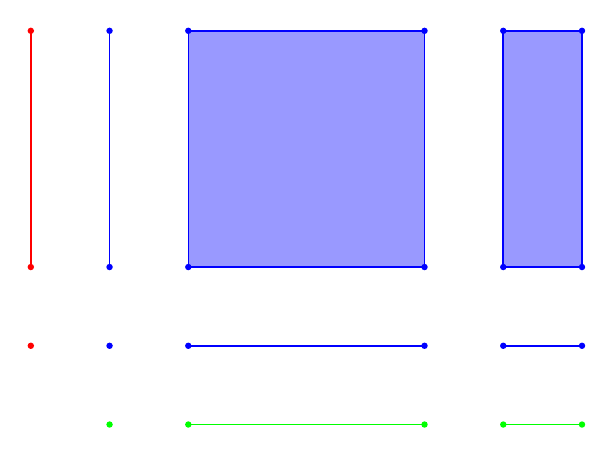
\begin{tikzpicture}[%
    >=Latex,
    line width=0.2mm,
    line cap=round
]

    % Draw green to indicate the set A.
    \begin{scope}[green]

        % Draw some points.
        \draw[fill=green] (1, 0) circle (0.3mm);
        \draw[fill=green] (2, 0) circle (0.3mm);
        \draw[fill=green] (5, 0) circle (0.3mm);
        \draw[fill=green] (6, 0) circle (0.3mm);
        \draw[fill=green] (7, 0) circle (0.3mm);

        % Draw lines.
        \draw (2, 0) to (5, 0);
        \draw (6, 0) to (7, 0);
    \end{scope}

    % Draw red to denote the set B.
    \begin{scope}[red]

        % Draw in some points.
        \draw[fill=red] (0, 1) circle (0.3mm);
        \draw[fill=red] (0, 2) circle (0.3mm);
        \draw[fill=red] (0, 5) circle (0.3mm);

        % Draw a line.
        \draw (0, 2) to (0, 5);
    \end{scope}

    % Use blue to mark AxB (Cartesian product).
    \begin{scope}[blue]

        % Fill in points.
        \draw[fill=blue] (1, 1) circle (0.3mm);
        \draw[fill=blue] (1, 2) circle (0.3mm);
        \draw[fill=blue] (1, 5) circle (0.3mm);
        \draw[fill=blue] (2, 1) circle (0.3mm);
        \draw[fill=blue] (5, 1) circle (0.3mm);
        \draw[fill=blue] (6, 1) circle (0.3mm);
        \draw[fill=blue] (7, 1) circle (0.3mm);
        \draw[fill=blue] (2, 2) circle (0.3mm);
        \draw[fill=blue] (2, 5) circle (0.3mm);
        \draw[fill=blue] (5, 2) circle (0.3mm);
        \draw[fill=blue] (5, 5) circle (0.3mm);
        \draw[fill=blue] (6, 2) circle (0.3mm);
        \draw[fill=blue] (7, 2) circle (0.3mm);
        \draw[fill=blue] (6, 5) circle (0.3mm);
        \draw[fill=blue] (7, 5) circle (0.3mm);

        % Draw lines.
        \draw (1, 2) to (1, 5);
        \draw (2, 1) to (5, 1);
        \draw (6, 1) to (7, 1);

        % Fill in rectangles.
        \draw[fill=blue, opacity=0.4] (2, 2) to (5, 2) to (5, 5)
                                             to (2, 5) to cycle;
        \draw[fill=blue, opacity=0.4] (6, 2) to (7, 2) to (7, 5)
                                             to (6, 5) to cycle;
        \draw (2, 2) to (5, 2) to (5, 5) to (2, 5) to cycle;
        \draw (6, 2) to (7, 2) to (7, 5) to (6, 5) to cycle;
    \end{scope}
\end{tikzpicture}
            \caption{Cartesian\_Product\_003.tex}
        \end{figure}
        \begin{figure}[H]
            \centering
            %--------------------------------Dependencies----------------------------------%
%   tikz                                                                       %
%       arrows.meta                                                            %
%       decorations.markings                                                   %
%-------------------------------Main Document----------------------------------%
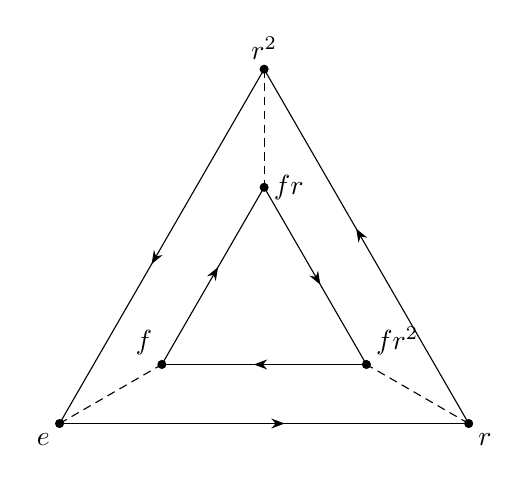
\begin{tikzpicture}[%
    ->-/.style={%
        decoration={%
            markings,
            mark=at position .55 with \arrow{Stealth}
        },
        postaction={decorate}
    }
]
    % The coordinates for the outter triangle.
    \coordinate (e)   at (210.0:3.0);
    \coordinate (r)   at (330.0:3.0);
    \coordinate (r2)  at (90.00:3.0);

    % The coordinates for the inner triangle.
    \coordinate (f)   at (210.0:1.5);
    \coordinate (fr2) at (330.0:1.5);
    \coordinate (fr)  at (90.00:1.5);

    % Dots for the coordinates.
    \foreach\x in {e,r,r2,f,fr,fr2}{%
        \draw[fill=black] (\x) circle (0.05);
    }

    % Solid arrows for rotations.
    \draw[->-] (e)   to (r);
    \draw[->-] (r)   to (r2);
    \draw[->-] (r2)  to (e);
    \draw[->-] (f)   to (fr);
    \draw[->-] (fr)  to (fr2);
    \draw[->-] (fr2) to (f);

    % Dashed arrows for reflections.
    \draw[densely dashed] (e)  to (f);
    \draw[densely dashed] (r)  to (fr2);
    \draw[densely dashed] (r2) to (fr);

    % Label the nodes.
    \node at (e)   [below left]  {$e$};
    \node at (r)   [below right] {$r$};
    \node at (r2)  [above]       {$r^{2}$};
    \node at (f)   [above left]  {$f$};
    \node at (fr)  [right]       {$fr$};
    \node at (fr2) [above right] {$fr^{2}$};
\end{tikzpicture}
            \caption{Cayley\_Diagram\_D6.tex}
        \end{figure}
        \begin{figure}[H]
            \centering
            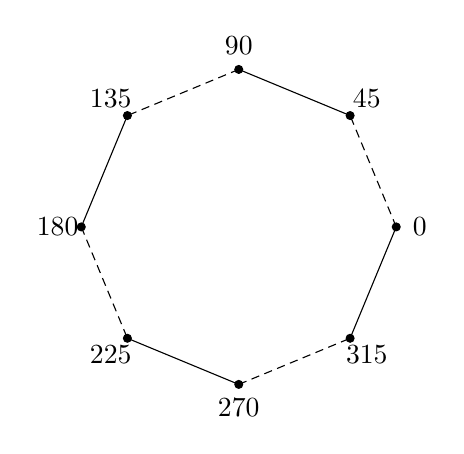
\begin{tikzpicture}
    % Coordinates for the points.
    \foreach\x in {0,45,90,135,180,225,270,315}{%
        \coordinate (\x) at (\x:2);
        \draw[fill=black] (\x) circle (0.05);
        \node at (\x:2.3) {$\x$};
    }

    % Dashed lines for acting by d.
    \draw[densely dashed] (0)   to (45);
    \draw[densely dashed] (90)  to (135);
    \draw[densely dashed] (180) to (225);
    \draw[densely dashed] (270) to (315);

    % Dashed lines for acting by d.
    \draw(45)  to (90);
    \draw(135) to (180);
    \draw(225) to (270);
    \draw(315) to (0);
\end{tikzpicture}
            \caption{Cayley\_Diagram\_D8\_Alt.tex}
        \end{figure}
        \begin{figure}[H]
            \centering
            %--------------------------------Dependencies----------------------------------%
%   tikz                                                                       %
%       arrows.meta                                                            %
%       decorations.markings                                                   %
%-------------------------------Main Document----------------------------------%
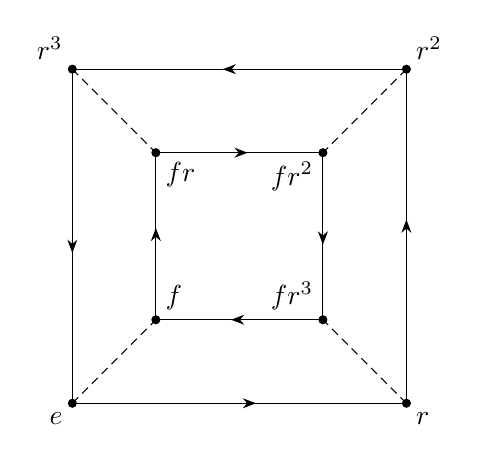
\begin{tikzpicture}[%
    ->-/.style={%
        decoration={%
            markings,
            mark=at position .55 with \arrow{Stealth}
        },
        postaction={decorate}
    }
]
    % Coordinates for the outter square.
    \coordinate (e)  at (225.0:3.0);
    \coordinate (r)  at (315.0:3.0);
    \coordinate (r2) at (45.00:3.0);
    \coordinate (r3) at (135.0:3.0);

    % Coordinates for inner square.
    \coordinate (fr2) at (45.00:1.5);
    \coordinate (fr)  at (135.0:1.5);
    \coordinate (f)   at (225.0:1.5);
    \coordinate (fr3) at (315.0:1.5);

    % Dots for the coordinates.
    \foreach\x in {e,r,r2,r3,f,fr,fr2,fr3}{%
        \draw[fill=black] (\x) circle (0.05);
    }

    % Solid arrows for rotations.
    \draw[->-] (e)   to (r);
    \draw[->-] (r)   to (r2);
    \draw[->-] (r2)  to (r3);
    \draw[->-] (r3)  to (e);
    \draw[->-] (f)   to (fr);
    \draw[->-] (fr)  to (fr2);
    \draw[->-] (fr2) to (fr3);
    \draw[->-] (fr3) to (f);

    % Dashed arrows for reflections.
    \draw[densely dashed] (e) to (f);
    \draw[densely dashed] (r) to (fr3);
    \draw[densely dashed] (r2) to (fr2);
    \draw[densely dashed] (r3) to (fr);

    % Label the points.
    \node at (e)   [below left]  {$e$};
    \node at (r)   [below right] {$r$};
    \node at (r2)  [above right] {$r^{2}$};
    \node at (r3)  [above left]  {$r^{3}$};
    \node at (f)   [above right] {$f$};
    \node at (fr3) [above left]  {$fr^{3}$};
    \node at (fr2) [below left]  {$fr^{2}$};
    \node at (fr)  [below right] {$fr$};
\end{tikzpicture}
            \caption{Cayley\_Diagram\_D8.tex}
        \end{figure}
        \begin{figure}[H]
            \centering
            %--------------------------------Dependencies----------------------------------%
%   tikz                                                                       %
%       arrows.meta                                                            %
%       decorations.markings                                                   %
%-------------------------------Main Document----------------------------------%
\begin{tikzpicture}[%
    ->-/.style={%
        decoration={%
            markings,
            mark=at position .55 with \arrow{Stealth}
        },
        postaction={decorate}
    }
]
    % Coordinates for the points.
    \foreach\x in {0,60,120,180,240,300}{%
        \coordinate (\x) at (\x:2);

        % Add dots for each point.
        \draw[fill=black] (\x) circle (0.05);

        % Label the points by their angle on the unit circle.
        \node at (\x:2.4) {$\x$};
    }

    % Dashed lines for acting by a.
    \draw[densely dashed] (0)   to (60);
    \draw[densely dashed] (120) to (180);
    \draw[densely dashed] (240) to (300);

    % Solid lines for acting by b.
    \draw[->-] (60)  to (120);
    \draw[->-] (180) to (240);
    \draw[->-] (300) to (0);
\end{tikzpicture}
            \caption{Cayley\_Diagram\_S3.tex}
        \end{figure}
        \begin{figure}[H]
            \centering
            \begin{tikzpicture}
    % Coordinates for the points.
    \coordinate (OO) at (0, 0);
    \coordinate (OI) at (0, 3);
    \coordinate (IO) at (3, 0);
    \coordinate (II) at (3, 3);

    % Dashed lines for +(0,1)
    \draw[densely dashed] (OO) to (OI);
    \draw[densely dashed] (IO) to (II);

    % Solid lines for +(1,0)
    \draw (OO) to (IO);
    \draw (OI) to (II);

    % Dots for the points.
    \draw[fill=black] (OO) circle (0.05);
    \draw[fill=black] (OI) circle (0.05);
    \draw[fill=black] (IO) circle (0.05);
    \draw[fill=black] (II) circle (0.05);

    % Labels for the points.
    \node at (OO) [below left]  {$(0,0)$};
    \node at (OI) [above left]  {$(0,1)$};
    \node at (IO) [below right] {$(1,0)$};
    \node at (II) [above right] {$(1,1)$};
\end{tikzpicture}
            \caption{Cayley\_Diagram\_Z2\_Z2.tex}
        \end{figure}
        \begin{figure}[H]
            \centering
            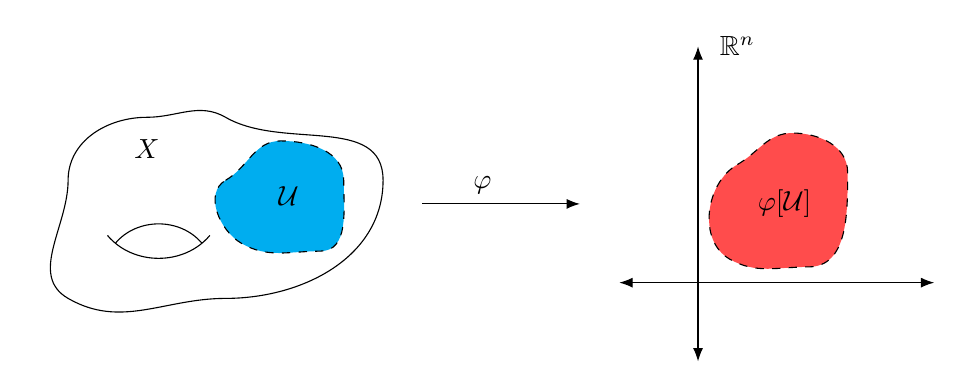
\begin{tikzpicture}[>=LaTeX]

    % Draw the coordinate axes for R^n.
    \draw[<->] (-1,  0) to (3, 0);
    \draw[<->] ( 0, -1) to (0, 3);

    % Red blob for the image of U.
    \draw[dashed, fill=red!70!white]
    (0.5, 1.5) to[out=30,  in=180]  (1.2,  1.9)
               to[out=0,   in=90]   (1.9,  1.4)
               to[out=-90, in=0]    (1.4,  0.2)
               to[out=180, in=-30]  (0.4,  0.3)
               to[out=150, in=-150] cycle;

    % Labels for R^n and the map phi.
    \node at (0.5, 3.0) {$\mathbb{R}^{n}$};
    \node at (1.1, 1.0) {$\varphi[\mathcal{U}]$};

    % Arrow representing the mapping phi.
    \draw[->] (-3.5, 1) to node[above left] {$\varphi$} (-1.5, 1);

    % Draw the manifolx X, shifted over to the left.
    \begin{scope}[xshift=-8cm,yshift=1.3cm]
        \draw (0,0) to[out=90,  in=180] (1,  0.8)
                    to[out=0,   in=150] (2,  0.8)
                    to[out=-30, in=90]  (4,  0.0)
                    to[out=-90, in=0]   (2, -1.5)
                    to[out=180, in=-30] (0, -1.5)
                    to[out=150, in=-90] cycle;
        
        % Add a donut hole in the manifold.
        \draw (0.5, -0.7) to[in=-130, out=-50] (1.8, -0.7);
        \draw (0.6, -0.8) to[in=130,  out=50]  (1.7, -0.8);

        % Draw a cyan blob for U.
        \draw[dashed, fill=cyan]
            (2.0, 0.0) to[out=30,  in=180]  (2.7,  0.5)
                       to[out=0,   in=90]   (3.5,  0.0)
                       to[out=-90, in=0]    (3.2, -0.9)
                       to[out=180, in=-30]  (2.2, -0.8)
                       to[out=150, in=-150] cycle;

        % Add some labels.
        \node at (2.8, -0.2) {$\mathcal{U}$};
        \node at (1.0,  0.4) {$X$};
    \end{scope}
\end{tikzpicture}
            \caption{Chart\_in\_a\_Manifold.tex}
        \end{figure}
        \begin{figure}[H]
            \centering
            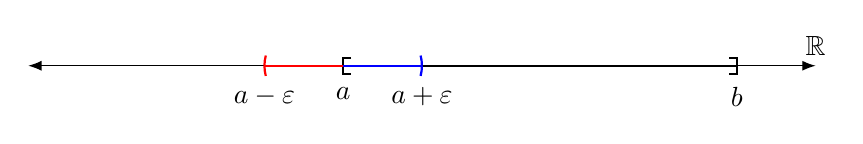
\begin{tikzpicture}[>=Latex]
    % Coordinates for various points.
    \coordinate (a)  at (4.0,  0.0);
    \coordinate (b)  at (9.0,  0.0);
    \coordinate (xl) at (3.0,  0.0);
    \coordinate (xr) at (5.0,  0.0);

    % Draw the real line.
    \draw[<->]   (0, 0) to (10, 0) node[above] {$\mathbb{R}$};

    % Draw the closed interval [a, b].
    \draw[thick] (a) to (b);

    % Add "brackets" indicating it is a closed interval.
    \draw[thick] (8.9, 0.1) to (9.0, 0.1) to (9.0, -0.1) to (8.9, -0.1);
    \draw[thick] (4.1, 0.1) to (4.0, 0.1) to (4.0, -0.1) to (4.1, -0.1);

    % Labels for the vaious points.
    \node at (a)  [below=1ex] {$a$};
    \node at (b)  [below=1ex] {$b$};
    \node at (xl) [below=1ex] {$a-\varepsilon$};
    \node at (xr) [below=1ex] {$a+\varepsilon$};

    % Draw the part of the open interval (a-e, a+e) that is inside of [a, b].
    \draw[blue, thick] (xr) arc (0:15:0.5);
    \draw[blue, thick] (xr) arc (0:-15:0.5);
    \draw[blue, thick] (a) to (xr);

    % Draw the part that falls outside.
    \draw[red, thick]  (xl) arc (180:195:0.5);
    \draw[red, thick]  (xl) arc (180:165:0.5);
    \draw[red, thick]  (a) to (xl);
\end{tikzpicture}
            \caption{Closed\_Interval\_in\_Not\_Open.tex}
        \end{figure}
        \begin{figure}[H]
            \centering
            %--------------------------------Dependencies----------------------------------%
%   amsfonts                                                                   %
%   tikz                                                                       %
%       arrows.meta                                                            %
%       positioning                                                            %
%       decorations.markings                                                   %
%-------------------------------Main Document----------------------------------%
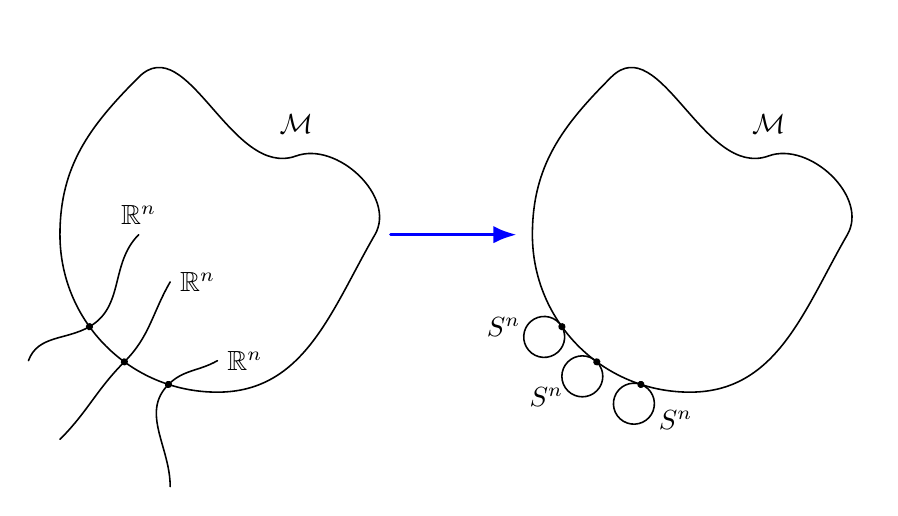
\begin{tikzpicture}[%
    >=latex,
    line width=0.2mm,
    line cap=round,
    scale=2
]

    % Coordinates for left blob.
    \coordinate (O1) at ( 0.0, 0.0);
    \coordinate (P1) at ( 1.0, 1.0);
    \coordinate (P2) at ( 0.5, 1.5);
    \coordinate (P3) at (-0.5, 2.0);
    \coordinate (P4) at (-1.0, 1.0);
    \coordinate (M1) at ( 0.5, 1.7);

    % Coordinates for right blob.
    \coordinate (O2) at (3.0, 0.0);
    \coordinate (Q1) at (4.0, 1.0);
    \coordinate (Q2) at (3.5, 1.5);
    \coordinate (Q3) at (2.5, 2.0);
    \coordinate (Q4) at (2.0, 1.0);
    \coordinate (M2) at (3.5, 1.7);

    % Squiggle one.
    \coordinate (L1) at (-1.2, 0.2);
    \coordinate (L2) at (-0.5, 1.0);

    % Squiggle two.
    \coordinate (L3) at (-1.0, -0.3);
    \coordinate (L4) at (-0.3,  0.7);

    % Squiggle three.
    \coordinate (L5) at (-0.3, -0.6);
    \coordinate (L6) at ( 0.0,  0.2);

    % Draw the left blob.
    \draw[%
        postaction={decorate},
        decoration={%
            markings,
            mark=at position .85 with 
                {\filldraw circle (1pt) coordinate (a);},
            mark=at position .9 with
                {\filldraw circle (1pt) coordinate (b);},
            mark=at position .95 with
                {\filldraw circle (1pt) coordinate (c);}
        }
    ]     (O1) to [out=0,in=-120]  (P1) to [out=60,in=20]   (P2)
               to [out=-160,in=45] (P3) to [out=-135,in=90] (P4)
               to [out=-90,in=180] cycle;

    % Label the left manifold as M.
    \node at (M1) {$\mathcal{M}$};

    % Draw squiggles through the three points.
    \draw (L1) to [out=70,in=-150] (a)
               to [out=30,in=-135] (L2) node[above] {$\mathbb{R}^{n}$};
    \draw (L3) to [out=45,in=-135] (b)
               to [out=45,in=-120] (L4) node[right] {$\mathbb{R}^{n}$};
    \draw (L5) to [out=90,in=-135] (c)
               to [out=45,in=-150] (L6) node[right] {$\mathbb{R}^{n}$};

    % Draw arrow from Manifold 1 to Manifold 2.        
    \draw[>=Latex, ->, blue, very thick] (1.1, 1.0) to (1.9, 1.0);

    % Draw right blob.
    \draw[%
        postaction={decorate},
        decoration={%
            markings,
            mark=at position .85 with 
                {\filldraw circle (1pt) coordinate (a);},
            mark=at position .9 with
                {\filldraw circle (1pt) coordinate (b);},
            mark=at position .95 with
                {\filldraw circle (1pt) coordinate (c);}
        }
    ]     (O2) to [out=0,in=-120]  (Q1) to [out=60,in=20] (Q2)
               to [out=-160,in=45] (Q3) to [out=-135,in=90] (Q4)
               to [out=-90,in=180] cycle;

    % Label for the 
    \node at (M2) {$\mathcal{M}$};
    \draw (a) arc(30:390:0.13) node[left=4mm] {$S^{n}$};
    \draw (b) arc(45:405:0.13) node[below left=2mm and 3mm] {$S^{n}$};
    \draw (c) arc(70:430:0.13) node[below right=2mm and 1mm] {$S^{n}$};
\end{tikzpicture}
            \caption{Compactification\_of\_Vector\_Bundle.tex}
        \end{figure}
        \begin{figure}[H]
            \centering
            %--------------------------------Dependencies----------------------------------%
%   amssymb                                                                    %
%   pgfplots                                                                   %
%       compat=1.9                                                             %
%   tikz                                                                       %
%       arrows.meta                                                            %
%   Unary minus sign.                                                          %
%       \DeclareMathSymbol{\minus}{\mathbin}{AMSa}{"39}                        %
%-------------------------------Main Document----------------------------------%
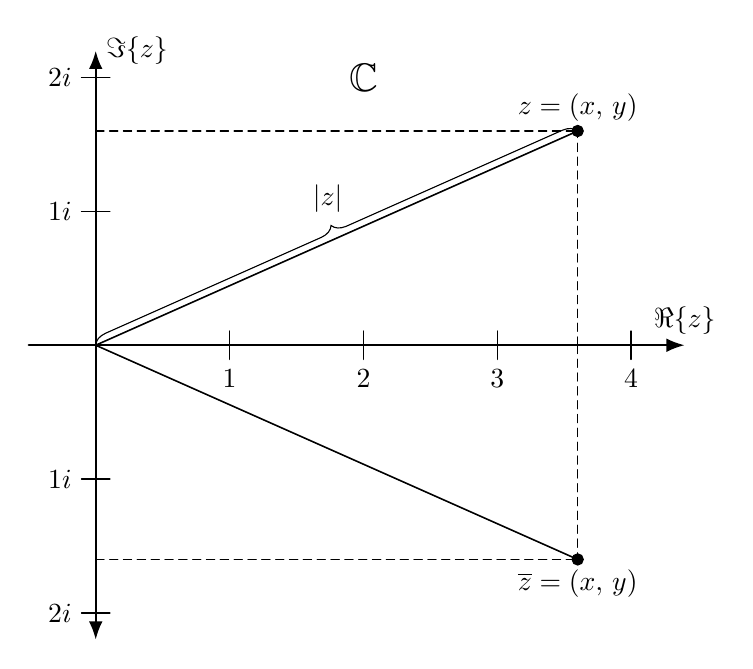
\begin{tikzpicture}[%
    >=Latex,
    line width=0.2mm,
    line cap=round,
    scale=1.7
]

    % Coordinates for the various points used.
    \coordinate (O)       at (0.0,  0.0);
    \coordinate (z_x)     at (3.6,  0.0);
    \coordinate (z_y)     at (0.0,  1.6);
    \coordinate (z)       at (3.6,  1.6);
    \coordinate (z_bar)   at (3.6, -1.6);
    \coordinate (z_bar_y) at (0.0, -1.6);
    \coordinate (C)       at (2.0,  2.0);

    % Axes:
    \begin{scope}[thick]
        \draw[->]  (-0.5,  0.0) to (4.4, 0) node [above] {$\Re\{z\}$};
        \draw[<->] ( 0.0, -2.2) to (0, 2.2) node [right] {$\Im\{z\}$};
    \end{scope}

    % Axes labels:
    \foreach\n in {1, 2}{%
        \draw (\n, 3pt)  to (\n, -3pt)  node [below] {$\n$};
        \draw (3pt, \n)  to (-3pt, \n)  node [left]  {$\n{i}$};
        \draw (3pt, -\n) to (-3pt, -\n) node [left]  {$\minus\n{i}$};
    }

    % More labels for the x-axis.
    \foreach\n in {3, 4}{%
        \draw (\n, 3pt) to (\n, -3pt) node [below] {$\n$};
    }

    % Draw a line from the origin to the point (x, y).
    \draw (O) to node [above left=2mm and -2mm] {$|z|$} (z);

    % Draw a brace denoting the magnitude of z.
    \draw[decorate, decoration={brace, amplitude=5pt},thin] (O) to (z);

    % Draw a line from the origin to the conjugate of z.
    \draw (O) to (z_bar);

    % Scope for dashed lines.
    \begin{scope}[densely dashed, thin]
        % Draw dashed lines for z.
        \draw[densely dashed, thin] (z_y) to (z);
        \draw[densely dashed, thin] (z_x) to (z);

        % Draw dashed lines for the conjugate of z.
        \draw[densely dashed, thin] (z_bar_y) to (z_bar);
        \draw[densely dashed, thin] (z_x)     to (z_bar);
    \end{scope}

    % Points for z and z_bar.
    \draw[fill=black] (z)     circle (0.4mm);
    \draw[fill=black] (z_bar) circle (0.4mm);

    % Nodes for labelling.
    \node at (C)              {\Large{$\mathbb{C}$}};
    \node at (z)     [above]  {$z=(x,\,y)$};
    \node at (z_bar) [below]  {$\overline{z}=(x,\,\minus{y})$};
\end{tikzpicture}
            \caption{Complex\_Number\_Conjugate\_and\_Modulus.tex}
        \end{figure}
        \begin{figure}[H]
            \centering
            %--------------------------------Dependencies---------------------------------%
%   amssymb                                                                   %
%   tikz                                                                      %
%       arrows.meta                                                           %
%-------------------------------Main Document---------------------------------%
\begin{tikzpicture}[%
    >=Latex,
    line width=0.2mm,
    line cap=round,
    scale=1.7
]

    % Coordinates for the various points.
    \coordinate (O)   at (0.0, 0.0);
    \coordinate (z)   at (2.3, 2.1);
    \coordinate (z_x) at (2.3, 0.0);
    \coordinate (z_y) at (0.0, 2.1);
    \coordinate (C)   at (3.0, 3.0);

    % Axes:
    \begin{scope}[thick]
        \draw[->] (-0.5,  0.0) to (4.4, 0.0) node [above] {$\Re\{z\}$};
        \draw[->] ( 0.0, -0.5) to (0.0, 4.4) node [right] {$\Im\{z\}$};
    \end{scope}

    % Axes labels:
    \foreach\n in {1,2,3,4}{%
        \draw (\n, 3pt) to (\n, -3pt) node [below] {$\n$};
        \draw (3pt, \n) to (-3pt, \n) node [left] {$\n{i}$};
    }

    % Draw a line from the origin to the point z.
    \draw (O) to (z);

    % Scope for dashed lines.
    \begin{scope}[densely dashed, thin]
        \draw (z_x) to (z);
        \draw (z_y) to (z);
    \end{scope}

    % Draw a point to denote z.
    \draw[fill=black] (2.3, 2.1) circle (0.4mm);

    % Nodes for labeling.
    \node at (C)          {\Large{$\mathbb{C}$}};
    \node at (z) [above]  {$z=(x,\,y)$};
\end{tikzpicture}

            \caption{Complex\_Plane\_Cartesian\_Representation.tex}
        \end{figure}
        \begin{figure}[H]
            \centering
            %--------------------------------Dependencies----------------------------------%
%   amssymb                                                                    %
%   tikz                                                                       %
%       arrows.meta                                                            %
%       decorations.markings                                                   %
%-------------------------------Main Document----------------------------------%
\begin{tikzpicture}[%
    line width=0.2mm,
    line cap=round,
    >=Latex,
    ->-/.style={%
        decoration={%
            markings,
            mark=at position 0.55 with \arrow{>},
        },
        postaction={decorate}
    },
    scale=1.7
]

    % Coordinates for points.
    \coordinate (O) at (0.0, 0.0);
    \coordinate (R) at (3.0, 0.0);
    \coordinate (P) at (2.12132, 2.12132);
    \coordinate (C) at (3.0, 3.0);
    \coordinate (G) at (1.0, 1.5);

    % Axes:
    \begin{scope}[thick]
        \draw[->] (-0.5, 0) to (4, 0) node[above] {$\Re\{z\}$};
        \draw[->] (0, -0.5) to (0, 4) node[right] {$\Im\{z\}$};
    \end{scope}

    % Axes Labels:
    \draw (3, 3pt) to (3, -3pt) node [below] {$R$};
    \draw (3pt, 3) to (-3pt, 3) node [left]  {$R$};

    % Draw the Jordan curve.
    \draw[->-, draw=blue] (O) to (R);
    \draw[->-, draw=blue] (P) to (O);
    \draw[->-, draw=blue] (R) arc (0:45:3);

    % Labels for various things.
    \node at (G) {$C_{R}(t)$};
    \node at (C) {\Large{$\mathbb{C}$}};
\end{tikzpicture}

            \caption{Complex\_Plane\_Fresnel\_Integral\_Path.tex}
        \end{figure}
        \begin{figure}[H]
            \centering
            %--------------------------------Dependencies----------------------------------%
%   amssymb                                                                    %
%   tikz                                                                       %
%       arrows.meta                                                            %
%   Int DeclareMathOperator                                                    %
%       \DeclareMathOperator{\Int}{Int}                                        %
%-------------------------------Main Document----------------------------------%
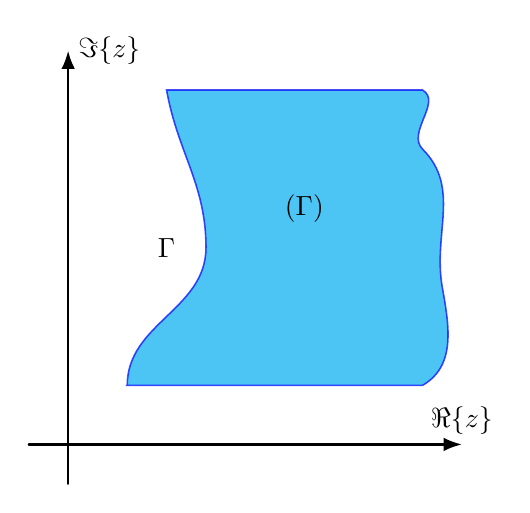
\begin{tikzpicture}[%
    >=Latex,
    line width=0.2mm,
    line cap=round,
    scale=2.5
]

    % Coordinates for the points that define the frame of the figure.
    \coordinate (P1) at (0.3, 0.3);
    \coordinate (P2) at (1.8, 0.3);
    \coordinate (P3) at (1.9, 0.8);
    \coordinate (P4) at (1.8, 1.5);
    \coordinate (P5) at (1.8, 1.8);
    \coordinate (P6) at (0.5, 1.8);
    \coordinate (P7) at (0.7, 1.0);

    % Axes:
    \begin{scope}[thick]
        \draw[->] (-0.2, 0) to (2, 0) node [above] {$\Re\{z\}$};
        \draw[->] (0, -0.2) to (0, 2) node [right] {$\Im\{z\}$};
    \end{scope}

    % Draw the simple region.
    \draw[blue,fill=cyan,opacity=0.7] (P1) to (P2)
        to [out=30,in=-80]  (P3)
        to [out=100,in=-45] (P4)
        to [out=135,in=-30] (P5)
        to                  (P6)
        to [out=-80,in=90]  (P7)
        to [out=-90,in=90]  cycle;

    % Nodes to label the Jordan curve and its interior.
    \node at (0.5,1)   {$\Gamma$};
    \node at (1.2,1.2) {$\Int(\Gamma)$};
\end{tikzpicture}

            \caption{Complex\_Plane\_Horizontally\_Simple.tex}
        \end{figure}
        \begin{figure}[H]
            \centering
            %--------------------------------Dependencies----------------------------------%
%   amssymb                                                                    %
%   tikz                                                                       %
%       arrows.meta                                                            %
%       angles                                                                 %
%       quotes                                                                 %
%-------------------------------Main Document----------------------------------%
\begin{tikzpicture}[%
    >=Latex,
    line width=0.2mm,
    line cap=round,
    scale=1.7
]

    % Coordinates for various points.
    \coordinate (O)   at (0.0, 0.0);
    \coordinate (z)   at (3.3, 1.6);
    \coordinate (z_x) at (3.3, 0.0);
    \coordinate (C)   at (4.0, 4.0);

    % Axes:
    \begin{scope}[thick]
        \draw[->] (-0.5,  0.0) to (4.4, 0.0) node [above] {$\Re\{z\}$};
        \draw[->] ( 0.0, -0.5) to (0.0, 4.4) node [right] {$\Im\{z\}$};
    \end{scope}

    % Axes labels:
    \foreach\n in {1, 2, 3, 4}{%
        \draw (\n, 3pt) to (\n, -3pt) node [below] {$\n$};
        \draw (3pt, \n) to (-3pt, \n) node [left] {$\n{i}$};
    }

    % Draw a line from the origin to the point z.
    \draw (O) to node [above] {$r$} (z);

    % Draw a dot marking the point z.
    \draw[fill=black] (z) circle (0.4mm);

    % Nodes to label various things.
    \node at (C) {\Large{$\mathbb{C}$}};
    \node at (z) [above] {$z=(r,\theta)$};
    \pic[%
        draw=black,
        "{${\theta}$}",
        angle eccentricity=1.2,
        angle radius=1.3cm
    ]   {angle = z_x--O--z};
\end{tikzpicture}

            \caption{Complex\_Plane\_Polar\_Form.tex}
        \end{figure}
        \begin{figure}[H]
            \centering
            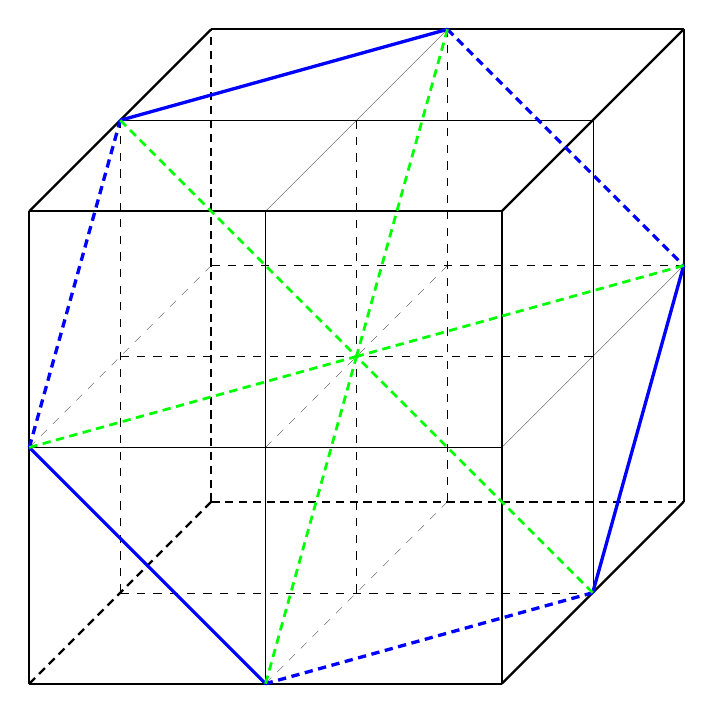
\begin{tikzpicture}

    % Lots of coordinates.
    \coordinate (O)   at (0, 0, 0);
    \coordinate (x)   at (6, 0, 0);
    \coordinate (y)   at (0, 6, 0);
    \coordinate (z)   at (0, 0, 6);
    \coordinate (xy)  at (6, 6, 0);
    \coordinate (xz)  at (6, 0, 6);
    \coordinate (yz)  at (0, 6, 6);
    \coordinate (xyz) at (6, 6, 6);
    \coordinate (MID) at (3, 3, 3);
    \coordinate (a1)  at (3, 0, 6);
    \coordinate (a2)  at (3, 6, 6);
    \coordinate (a3)  at (0, 3, 6);
    \coordinate (a4)  at (6, 3, 6);
    \coordinate (b1)  at (0, 0, 3);
    \coordinate (b2)  at (6, 0, 3);
    \coordinate (b3)  at (a1);
    \coordinate (b4)  at (3, 0, 0);
    \coordinate (c1)  at (b2);
    \coordinate (c2)  at (6, 6, 3);
    \coordinate (c3)  at (a4);
    \coordinate (c4)  at (6, 3, 0);
    \coordinate (d1)  at (0, 6, 3);
    \coordinate (d2)  at (c2);
    \coordinate (d3)  at (a2);
    \coordinate (d4)  at (3, 6, 0);
    \coordinate (e1)  at (a3);
    \coordinate (e2)  at (0, 3, 0);
    \coordinate (e3)  at (b1);
    \coordinate (e4)  at (d1);
    \coordinate (f1)  at (e2);
    \coordinate (f2)  at (c4);
    \coordinate (f3)  at (b4);
    \coordinate (f4)  at (d4);
    \coordinate (A) at (3, 3, 6);
    \coordinate (B) at (3, 0, 3);
    \coordinate (C) at (6, 3, 3);
    \coordinate (D) at (3, 6, 3);
    \coordinate (E) at (0, 3, 3);
    \coordinate (F) at (3, 3, 0);

    % Draw the cube.
    \begin{scope}[thick]
        \draw[densely dashed] (O) to (x);
        \draw[densely dashed] (O) to (y);
        \draw[densely dashed] (O) to (z);
        \draw (x)  to (xy);
        \draw (y)  to (xy);
        \draw (x)  to (xz);
        \draw (z)  to (xz);
        \draw (y)  to (yz);
        \draw (z)  to (yz);
        \draw (xy) to (xyz);
        \draw (yz) to (xyz);
        \draw (xz) to (xyz);
    \end{scope}

    % Some dashed lines inside the cube.
    \begin{scope}[line width=0.1pt]
        \draw (a1) to (a2);
        \draw (a3) to (a4);
        \draw[dashed] (b1) to (b2);
        \draw[dashed] (b3) to (b4);
        \draw (c1) to (c2);
        \draw (c3) to (c4);
        \draw (d1) to (d2);
        \draw (d3) to (d4);
        \draw[dashed] (e1) to (e2);
        \draw[dashed] (e3) to (e4);
        \draw[dashed] (f1) to (f2);
        \draw[dashed] (f3) to (f4);
        \draw[dashed] (A)  to (MID);
        \draw[dashed] (B)  to (MID);
        \draw[dashed] (C)  to (MID);
        \draw[dashed] (D)  to (MID);
        \draw[dashed] (E)  to (MID);
        \draw[dashed] (F)  to (MID);
    \end{scope}

    % Draw the hexagon.
    \begin{scope}[very thick, blue]
        \draw(a1) to (a3);
        \draw[densely dashed] (a3) to (d1);
        \draw (d1) to (d4);
        \draw[densely dashed] (d4) to (c4);
        \draw (c4) to (b2);
        \draw[densely dashed] (b2) to (a1);
    \end{scope}

    % Connect vertices to center of cube.
    \begin{scope}[densely dashed, green, line width=1pt]
        \draw (a1) to (MID);
        \draw (a3) to (MID);
        \draw (d1) to (MID);
        \draw (c4) to (MID);
        \draw (d4) to (MID);
        \draw (b2) to (MID);
    \end{scope}
\end{tikzpicture}
            \caption{Dipping\_a\_Cube\_in\_Water.tex}
        \end{figure}
        \begin{figure}[H]
            \centering
            \documentclass[crop,class=article]{standalone}
%----------------------------Preamble-------------------------------%
\usepackage{tikz}                       % Drawing/graphing tools.
\usetikzlibrary{arrows.meta}            % Latex arrows.
%--------------------------Main Document----------------------------%
\begin{document}
    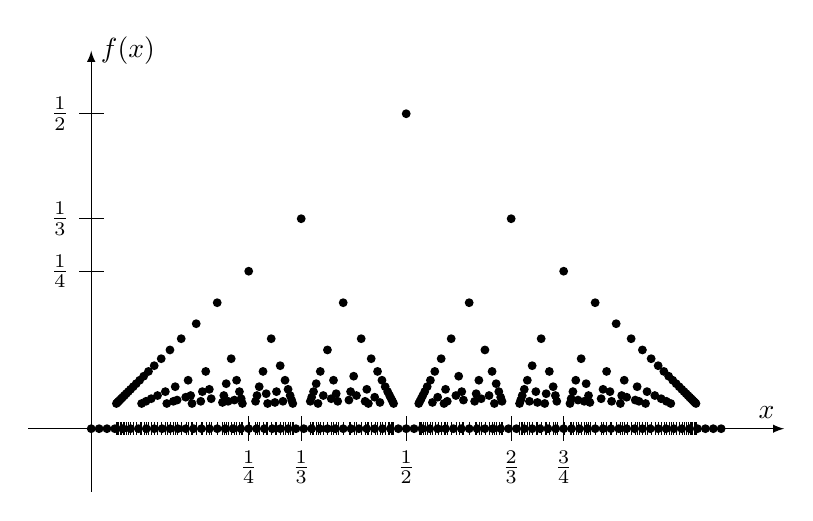
\begin{tikzpicture}[scale=8,>=latex]
        \draw[->] (-0.1,0) -- (1.1,0)
            node[above left] {$x$};
        \draw[->] (0,-0.1) -- (0,0.6)
            node[right] {$f(x)$};
        \draw (0.02,1/2) -- (-0.02,1/2)
            node[left]{$\frac{1}{2}$};
        \draw (0.02,1/3) -- (-0.02,1/3)
            node[left]{$\frac{1}{3}$};
        \draw (0.02,1/4) -- (-0.02,1/4)
            node[left]{$\frac{1}{4}$};
        \foreach\X[%
            evaluate=\X as \Ymax using {int(\X-1)}]
            in {25,24,...,2}{%
                \foreach\Y in {1,...,\Ymax}{%
                    \ifnum\X<5
                        \draw
                        (\Y/\X,0.02) -- (\Y/\X,-0.02)
                        node[below,fill=white]
                            {$\frac{\Y}{\X}$};
                    \else
                        \draw[ultra thin]
                        (\Y/\X,0.01) to (\Y/\X,-0.01);
                    \fi
                    \pgfmathtruncatemacro{\TST}
                        {gcd(\X,\Y)}
                    \ifnum\TST=1
                        \fill ({\Y/\X},1/\X) 
                            circle (0.2pt); 
                    \fi
                }
        }
        \foreach\X in {0,1,...,80}
        {\fill (\X/80,0) circle(0.2pt);}
    \end{tikzpicture}
\end{document}
            \caption{Dirichlet\_Popcorn\_Function.tex}
        \end{figure}
    \section{Asymptote}
        \begin{figure}[H]
            \centering
            \includegraphics{images/Heaviside.pdf}
            \caption{Heaviside.asy}
        \end{figure}
        \begin{figure}[H]
            \centering
            \includegraphics{images/Klein_Bottle.pdf}
            \caption{Klein\_Bottle.asy}
        \end{figure}
        \begin{figure}[H]
            \centering
            \includegraphics{images/Mobius_Strip.pdf}
            \caption{Mobius\_Strip.asy}
        \end{figure}
        \begin{figure}[H]
            \centering
            \includegraphics{images/Real_Projective_Plane.pdf}
            \caption{Real\_Projective\_Plane.asy}
        \end{figure}
        \begin{figure}[H]
            \centering
            \includegraphics{images/Sea_Shell.pdf}
            \caption{Sea\_Shell.asy}
        \end{figure}
        \begin{figure}[H]
            \centering
            \includegraphics{images/Seifert_Hopf_Link.pdf}
            \caption{Seifert\_Hopf\_Link.asy}
        \end{figure}
        \begin{figure}[H]
            \centering
            \includegraphics{images/Seifert_Trefoil.pdf}
            \caption{Mobius\_Strip.asy}
        \end{figure}
        \begin{figure}[H]
            \centering
            \includegraphics{images/Sphere_to_Disk_Homeo.pdf}
            \caption{Sphere\_to\_Disk\_Homeo.asy}
        \end{figure}
        \begin{figure}[H]
            \centering
            \includegraphics{images/Trefoil_Knot.pdf}
            \caption{Trefoil\_Knot.asy}
        \end{figure}
        \begin{figure}[H]
            \centering
            \includegraphics{images/Trefoil_Non_Oriented_Surface.pdf}
            \caption{Trefoil\_Non\_Oriented\_Surface.asy}
        \end{figure}
        \begin{figure}[H]
            \centering
            \includegraphics{images/Trefoil_Tricolor.pdf}
            \caption{Trefoil\_Tricolor.asy}
        \end{figure}
    \section{C Programming Language}
        \begin{figure}[H]
            \centering
            \resizebox{\textwidth}{!}{
                \includegraphics{images/NewtonRootsCubic.png}
            }
            \caption{Newton\_Fractal\_Cubic.c}
        \end{figure}
        \begin{figure}[H]
            \centering
            \resizebox{\textwidth}{!}{
                \includegraphics{images/NewtonRootsQuartic.png}
            }
            \caption{Newton\_Fractal\_Quartic.c}
        \end{figure}
        \begin{figure}[H]
            \centering
            \resizebox{\textwidth}{!}{
                \includegraphics{images/Mandelbrot.png}
            }
            \caption{Mandelbrot.c}
        \end{figure}
\end{document}